\documentclass{article}
\usepackage[left=2cm, right=2cm, top=0cm]{geometry}
\usepackage{amsmath}
\usepackage{amssymb}
\usepackage{graphicx}
\usepackage{tikz}
\usepackage{comment}
\usepackage{enumitem}
\usepackage{float}
\usepackage{hyperref}
\usepackage[margin=2cm]{caption}
\setlength\parindent{0pt}
\hypersetup{
    colorlinks,
    citecolor=green,
    filecolor=black,
    linkcolor=blue,
    urlcolor=blue
}

\begin{document}
\title{Assignment 1: Unconstrained Optimization}
\author{Jacob Puthipiroj}
%\date{}
\maketitle

Consider a drainage channel made with a single sheet of metal. The channel is open on top and is required to carry the largest amount of water possible. We wish to compute the base width of the channel $b$, as well as the angle $\theta$ at which the sides should be bent upwards in order to maximize the cross-sectional area.  We assume the width of the metal sheet is $W = 3$m, so we require $2a+b=W$.

\section*{Problem Setup}
First, we compute an expression for the cross-sectional area of the channel $A$ as a function of the base length $b$ and the angle at which the sides are bent upwards $\theta$. \\

We know the vertical height of the cross-section to be $a \sin \theta$. Similarly, the area jutting out beneath the bent sides are $a \cos\theta$ on both sides. Furthermore, we know $2a+b=3 \implies a = \frac{3 - b}{2}$. 
This gives the total area as 
$$ A(b,\theta) = ab \sin(\theta) + a^2 \sin(\theta)  \cos(\theta)  = a \sin(\theta) \big(b+a\cos (\theta) \big) = \frac{1}{4}(b-3) \sin(\theta) \big((b-3)\cos(\theta) - 2b \big)$$
%$$ A(b,\theta) = ab \sin\theta + a \sin\theta  \cos\theta  = a \sin\theta \big(b+\cos \theta \big) = \frac{3-b}{2} \sin\theta \big(b + \cos\theta \big)$$
Plotting the function over the domain $b \in [0, 3], \theta \in [0, \pi/2]$ gives the following:

\begin{figure*}[h]
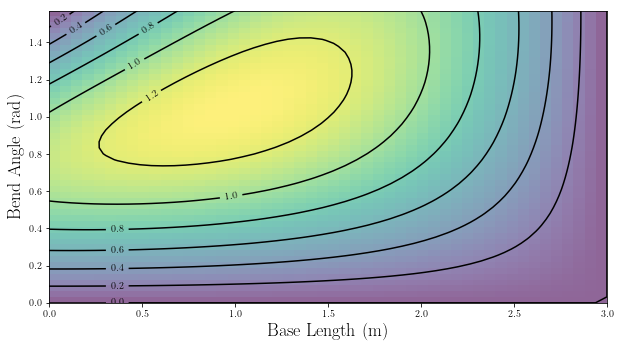
\includegraphics[scale = 0.43]{2dplot.png}
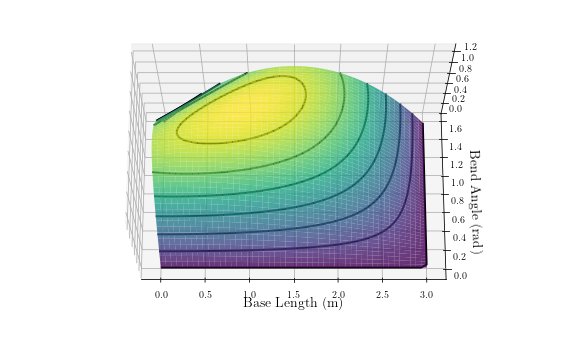
\includegraphics[trim = {3cm, 1cm, 3cm, 1.5cm}, clip, scale = 0.53]{3dplot.png}
\caption{The contour plots, as well as the 3D projection plot indicates that there is a unique maximum over the domain. This is critical point is approximately $x^* \approx [1 \textrm{m},1 \ \textrm{rad} ]$.}
\end{figure*}




%\begin{figure}[ht!]
% \centering
% 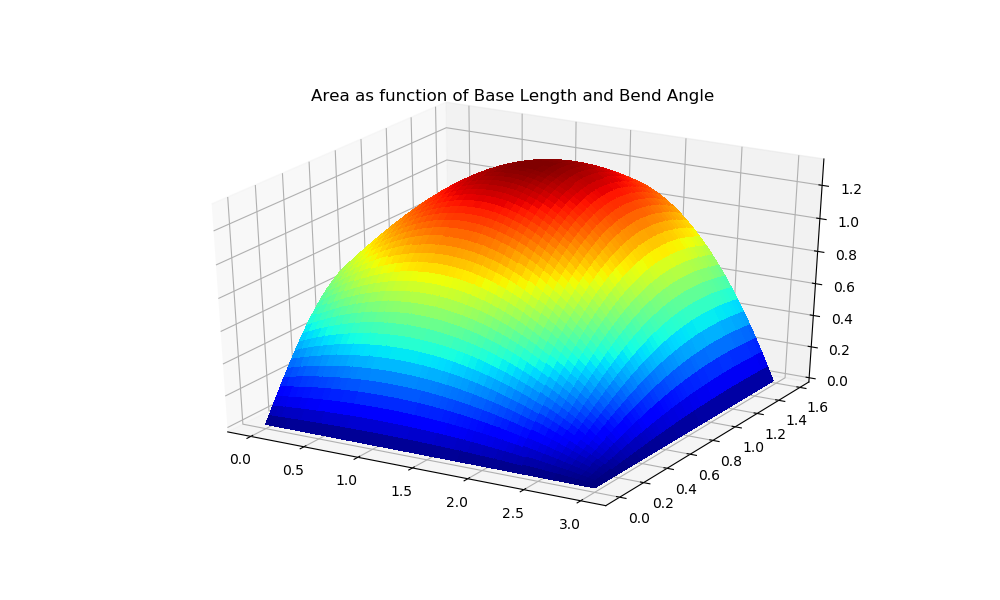
\includegraphics[scale = 0.5]{Channelplot.png}
%\end{figure}

\newgeometry{left=2cm, right=2cm}
\newpage
\section*{Analytical Solution}
We attempt to find the exact solution analytically via multivariable calculus. We have the objective  as
%$$A(b,\theta) = \frac{3-b}{2} \sin\theta \big(b + \cos\theta \big)$$
$$\frac{1}{4}(b-3) \sin(\theta) \big((b-3)\cos(\theta) - 2b \big)$$
For which the gradient is 0:
$$ \nabla A(b,\theta) = \bigg(\frac{\partial A}{\partial b}, \frac{\partial A}{\partial \theta} \bigg) = \bigg(\frac{1}{2} \sin \theta \big(3 - 2b - (3-b)\cos \theta),  \frac{3-b}{4} \big (\cos \theta (2b + (3-b)\cos \theta ) - (3-b) \sin^2 \theta \big)  \bigg)$$

Setting the first expression to 0 gives
$$ \frac{1}{2} \sin \theta \big(3 - 2b - (3-b)\cos \theta) = 0 \implies b = \frac{3 \cos \theta  - 3}{\cos \theta - 2}$$
And the second to 0 gives 
$$  \frac{3-b}{4} \big (\cos \theta (2b + (3-b)\cos \theta ) - (3-b) \sin^2 \theta \big) =0  \implies b = 3, \ b = -\frac{3\cos^2 \theta - 3 \sin^2 \theta}{2 \cos \theta 	- \cos^2 \theta + \sin ^2 \theta}$$
Then solving for equivalence of both right-hand equations:
$$ -\frac{3\cos^2 \theta - 3 \sin^2 \theta}{2 \cos \theta 	- \cos^2 \theta + \sin ^2 \theta} = \frac{3 \cos \theta  - 3}{\cos \theta - 2} \implies \cos \theta = \frac{1}{2} \implies b = 1,  \ \theta = \frac{\pi}{3} $$
% \qquad \theta \neq \frac{\pi}{2}(2n + 1) , n \in \mathbb{Z}$$
This should correspond to the maximum, and can be rigorously proven using the second derivative test. The Hessian is computed as
$$ H(b,\theta) = \begin{bmatrix} f_{xx}(x,y) & f_{xy}(x,y)\\ f_{yx}(x,y) & f_{yy}(x,y) \end{bmatrix} \implies H \big( 1, \pi/3 \big) = \begin{bmatrix} -0.64952 & 0.75 \\ 0.75 & -2.59807 \end{bmatrix}, \ \det \big( H(1, \pi/3) \big)=1.125$$ 
Since the Hessian is negative definite, we know $A$ attains a local maximum at $(1, \pi/3)$. 
%\begin{bmatrix} \frac{1}{4}\sin 2 \theta - \sin \theta & \frac{b-3}{2}\cos 2 \theta -(b-\frac{3}{2})\cos \theta \\ 
%\frac{1}{2}((3-2b)\cos \theta - (b-3)
%) & \frac{3-b}{2}() \end{bmatrix}$$
 
 \newpage

\section*{Numerical Solution}

\begin{figure*}[h]
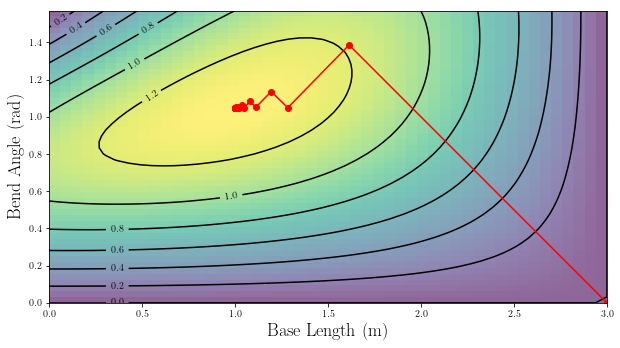
\includegraphics[scale = 0.43]{2dplotoptimized.png}
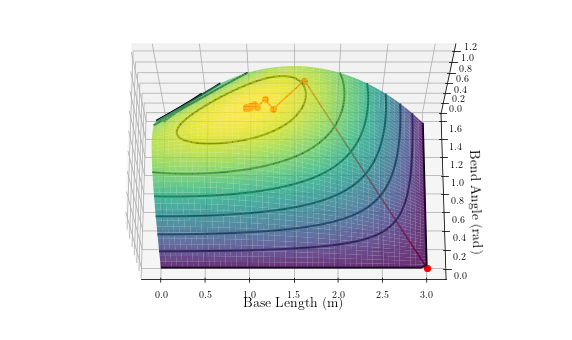
\includegraphics[trim = {3cm, 1cm, 3cm, 1.5cm}, clip, scale = 0.53]{3dplotoptimized.png}
\caption{We attempt to find the solution via gradient descent from the initial state (3,0). The line takes a zigzag pattern, as the steps are all orthogonal to each other. }
\end{figure*}
The numerical solution is done in Python using gradient descent, with code provided in the appendix. Unsurprisingly, we attain the same solution as with the analytical solution. We implement gradient descent, which is of the form 
$$ x_{n+1} = x_n - \alpha \nabla F(x_n)$$
Where each step of size $\alpha$ is taken in the direction of steepest descent, or $\nabla F$, and $\alpha$ is determined using bisection line search.
\newgeometry{left=2cm, right=2cm}



\section*{Appendix}
The code used for the numerical solutionis available \href{https://github.com/thetruejacob/CS164/blob/master/Exact%20Line%20Search.ipynb}{here}.
\subsection*{Line Search Algorithm}
\begin{verbatim}
	import numpy as np
from scipy.optimize import approx_fprime
from numpy.linalg import norm

def func(x):
    return 0.5 * (3-x[0]) * np.sin(x[1]) * (x[0] + 0.5 * (3-x[0]) * np.cos(x[1]))

def bisection(func, x0, maxiter = 10000):
    eps = np.sqrt(np.finfo(float).eps)  
    
    iters = 0  
    x = np.array(x0, dtype=float)
    xs, fs, alphs = x, np.array([func(x)]), np.array([0])
    
    grad = np.ones_like(x)
    
    while norm(grad) > 1e-4 and iters <= maxiter:
        grad = approx_fprime(x, func, eps)
        h = lambda a: -func(x + a*grad)
        
        upper, lower = np.array([0.001]), 0
        
        while approx_fprime(upper, h, eps) <= 0:upper *= 2
        while abs(approx_fprime(((upper + lower)/2), h, eps)) > 1e-6:
            if approx_fprime((upper + lower)/2, h, eps) > 0: upper = (upper + lower)/2
            else: lower = (upper + lower)/2
        
        xs, fs, alphs = np.vstack((xs, x)), 
        				np.vstack((fs, func(x))), 
        				np.vstack((alphs, (upper + lower) / 2))
        
        x += (upper + lower) / 2*grad
        iters += 1
    
    return(xs, fs, alphs)
\end{verbatim}


\begin{comment}
\subsection*{Analytical Solution - Finding $\theta$}
\begin{align*}
	\frac{3 - \cos \theta}{2} &= \frac{\sin^2 \theta }{\cos \theta} - \cos \theta \\
	0 &= \frac{1}{2}(3 - \cos \theta ) + \cos \theta  - \frac{\sin^2 \theta}{\cos \theta} \\
	0 &= \frac{\cos \theta (3- \cos \theta)}{2 \cos \theta} + \frac{2\cos^2 \theta }{2\cos \theta} - \frac{2 \sin^2 \theta}{2 \cos \theta }\\
	0 &= 3 \cos \theta + \cos^2 \theta - 2 \sin^2 \theta  \\
		0 &= 3 \cos^2 \theta + 3 \cos \theta. - 2 \\
	\cos\theta &= \frac{-3 \pm \sqrt{33}}{6} \\
	\theta &= \arccos \frac{-3 + \sqrt{33}}{6} + 2 \pi n, \theta = 2\pi - \arccos \frac{-3 + \sqrt{33}}{6} + 2 \pi n; \qquad n \in \mathbb{Z}
	\end{align*}
\end{comment}

\newpage
\section*{Convergence}
\begin{table}[h]
\begin{tabular}{|l|ll|l|l|}
\hline
Iteration & \multicolumn{1}{l|}{Base Length} & Bend Angle & Area     & New Step Size \\ \hline
0         & 2.999900                         & 0.000100   & 0.000000 & 9240.576000   \\ \hline
1         & 1.613860                         & 1.386163   & 1.186193 & 1.390922      \\ \hline
2         & 1.284212                         & 1.048693   & 1.273076 & 0.484234      \\ \hline
3         & 1.195211                         & 1.135630   & 1.289321 & 1.193750      \\ \hline
4         & 1.113347                         & 1.051817   & 1.295210 & 0.447375      \\ \hline
5         & 1.081791                         & 1.082634   & 1.297396 & 1.148000      \\ \hline
6         & 1.049737                         & 1.049819   & 1.298321 & 0.434750      \\ \hline
7         & 1.036507                         & 1.062748   & 1.298716 & 1.128000      \\ \hline
8         & 1.022611                         & 1.048527   & 1.298892 & 0.430000      \\ \hline
9         & 1.016715                         & 1.054269   & 1.298971 & 1.120000      \\ \hline
10        & 1.010432                         & 1.047830   & 1.299007 & 0.432000      \\ \hline
11        & 1.007708                         & 1.050486   & 1.299024 & 1.024000      \\ \hline
12        & 1.005095                         & 1.047675   & 1.299031 & 0.448000      \\ \hline
13        & 1.003772                         & 1.048828   & 1.299035 & 0.768000      \\ \hline
14        & 1.002827                         & 1.047751   & 1.299036 & 0.512000      \\ \hline
15        & 1.002099                         & 1.048100   & 1.299037 & 1.024000      \\ \hline
16        & 1.001395                         & 1.047312   & 1.299038 & 0.256000      \\ \hline
\end{tabular}
\end{table}
\end{document}